\documentclass[11pt,a4paper]{article}
\usepackage[utf8]{inputenc}
\usepackage[T1]{fontenc}
\usepackage{amsmath,amssymb,amsthm,mathtools}
\usepackage{geometry}
\usepackage{booktabs}
\usepackage{graphicx}
\usepackage{hyperref}

\geometry{margin=0.95in}
\emergencystretch=1.5em

\newtheorem{theorem}{Theorem}[section]
\newtheorem{proposition}[theorem]{Proposition}
\newtheorem{lemma}[theorem]{Lemma}
\newtheorem{corollary}[theorem]{Corollary}
\theoremstyle{definition}
\newtheorem{definition}[theorem]{Definition}
\newtheorem{remark}[theorem]{Remark}

\title{\textbf{Pillar 10: Clifford-Holonomy \& Cohomological Complexity Theory --- The Coboundary--Frustration Dichotomy, $\mathrm{Spin}(4)$ Gram Obstructions, and HONHSE Witness Funneling for $\mathbf{P}$ vs.\ $\mathbf{NP}$}}
\author{Mathematical Physics \& Quasicrystal Research Program \\ \small Theoretical \& Computational Physics Division}
\date{October 18, 2026}

\begin{document}
\maketitle

\begin{abstract}
We extend the discrete-geometric, gauge-theoretic, and non-Hermitian spectral framework of the \texttt{Chair44} and $6\mathrm{D}\to 3\mathrm{D}$ quasicrystal program to computational complexity theory and Constraint Satisfaction Problems (Bounded Polycube Tiling and Boolean $k$-SAT). First, we establish the \textbf{Coboundary--Holonomy Complexity Dichotomy}: whenever local constraint operators on a graph factor as a discrete $0$-cochain coboundary $V_{ab} = M_a^\top M_b \in \mathrm{SO}(3,\mathbb{Z})$ (the gauge-theoretic structure of $2$-SAT, affine XOR-SAT, and unfrustrated tree connections), every closed cycle has trivial Wilson loop holonomy $W_{\mathrm{vertex}}(\mathcal{C}) = I_3$, and single-pass tree propagation constructs a global satisfying assignment in linear time $\mathcal{O}(|V|+|E|) \in \mathbf{P}$. Conversely, when $3$-body clauses or polyhedral face panels couple vertex states to shared boundary normals via the Clifford connection $C_{ab}^{(f)} = (\boldsymbol{\sigma}\cdot\mathbf{u}_a)(\boldsymbol{\sigma}\cdot\mathbf{u}_b) \in Q_8$, non-abelian Wilson loops ($\mathrm{Tr}\,W = 0$) and central $\mathbb{Z}_2$ frustrations ($W = -I_2$) emerge. We prove by exhaustive machine-checked enumeration over all $8^3 = 512$ local spinor gauge transformations $(G_0,G_1,G_2)\in Q_8^3$ that no local vertex gauge transformation can trivialize a frustrated $3$-cycle, and establish unconditional restricted-model lower bounds: $2^{n-1}$/$2^n$ size lower bounds for $\mathrm{DNF}$, $\mathrm{CNF}$, and bottom-fan-in-$1$ $\Sigma_3$/$\Pi_3$ circuits; $2n$ literal and read-once impossibility bounds for unbounded-fan-in Depth-$2$ and Depth-$3$ circuits; and $2^n$ leaf/state-space lower bounds for decision trees, two-stage OBDDs, and Cook--Reckhow Resolution vs.\ $\mathcal{O}(m)$ degree-$1$ algebraic refutations (\texttt{XORProof}, \texttt{PCProof}, \texttt{CPProof}). Second, we prove that puncturing the $(1,1,1)$ octant to form the $3\mathrm{D}$ Chair $C_3 = [0,2]^3\setminus(1,2]^3$ removes the $8$th clause obstruction on $\{0,1\}^3$, creating a unique satisfying witness corner and enabling $2$-adic Schur-complement mode decoupling $\det(\lambda I_8 - L_{\mathrm{tile},1}) = (\lambda - 24)\det(\lambda I_7 - L_{\mathrm{eff}})$, whereas in $4\mathrm{D}$ ($C_4$) the $64\times 6$ $\mathrm{Spin}(4)$ boundary bivector matrix $\mathcal{M}_{\mathrm{obs}}$ has full rational rank $6$ with exact Gram determinant $\det(\mathcal{M}_{\mathrm{obs}}^\top \mathcal{M}_{\mathrm{obs}}) = 21{,}414{,}742 > 0$, providing an exact algebraic UNSAT certificate ($\dim\ker\mathcal{M}_{\mathrm{obs}} = 0$). Third, we construct a three-stage physical/spectral solver combining $2$-adic Schur renormalization, combinatorial $1$-form Hodge-Laplacian ($\Delta_1$) Hellmann--Feynman bottleneck repair, and Higher-Order Non-Hermitian Skin Effect (HONHSE) witness funneling on the Boolean hypercube $Q_n = \{0,1\}^n$, achieving a $52.33\times$ Inverse Participation Ratio (IPR) gain and $110.20\times$ witness probability amplification at $n=8$ with zero false-positive SAT claims ($\mathrm{FPR}_{\mathrm{pre}} = 0.0\%$ vs.\ $\mathrm{FPR}_{\mathrm{peek}} = 78.36\%$). All theorems are machine-checked in Lean~4 (\path{certificates/PvsNPCliffordCertificates.lean}, $76$ sections, $14{,}527$ lines, $440$ \texttt{\#print axioms} checks) and SymPy/Python (\path{src/cross_disciplinary/pillar10_p_vs_np_clifford_complexity.py}).
\end{abstract}

\section{The Coboundary--Holonomy Dichotomy: Tractable $\mathbf{P}$ vs.\ Non-Abelian $Q_8$ Frustration}

Both Cook's theorem ($3$-SAT) and Levin's theorem (Bounded Domino/Polycube Tiling) reduce arbitrary $\mathbf{NP}$ decision predicates to deciding whether local compatibility constraints over a cellular complex $\mathcal{K} = (V, E, F)$ admit a global section. Within the \texttt{Chair44} gauge framework, this question splits along an exact cohomological boundary.

\begin{theorem}[Coboundary Tractability in $\mathbf{P}$ vs.\ Exhaustive $Q_8$ Gauge No-Go Barrier]
\label{thm:dichotomy}
\leavevmode
Let $\mathcal{K} = (V, E, F)$ be a finite polyhedral constraint complex with vertex state space $G$.
\begin{enumerate}
    \item \textbf{Coboundary Regime ($\in \mathbf{P}$):} If the edge compatibility operators factor as a discrete $0$-cochain coboundary $V_{ab} = M_a^\top M_b \in \mathrm{SO}(3,\mathbb{Z})$ (or $d_0 x = b$ over $\mathbb{F}_2$), then along every closed cycle $\mathcal{C} = (v_0, v_1, \dots, v_m = v_0)$, the path-ordered Wilson loop telescopes identically to $W_{\mathrm{vertex}}(\mathcal{C}) = I_3$. Single-pass tree propagation $M_a = M_0 V_{0a}$ from a root vertex $v_0$ recovers the exact global satisfying assignment in $\mathcal{O}(|V|+|E|)$ linear time without backtracking.
    \item \textbf{Non-Abelian Clifford $Q_8$ Plaquette Obstruction:} On a $2$-complex where $3$-body clauses or shared panels $f \in F$ couple vertex frames to face normals $\mathbf{n}_f$ via $C_{ab}^{(f)} = (\boldsymbol{\sigma}\cdot \mathbf{u}_a^{(f)})(\boldsymbol{\sigma}\cdot \mathbf{u}_b^{(f)}) \in Q_8$, a frustrated $3$-cycle with base holonomy $W(\mathcal{C}) = q_k$ ($\mathrm{Tr}\,W = 0$) or central frustration $W(\mathcal{C}) = -I_2$ ($\mathrm{Tr}\,W = -2$) satisfies across all $|Q_8^3| = 512$ local spinor gauge transformations:
    \begin{equation}
    \forall (G_0, G_1, G_2) \in Q_8^3 : \quad W'(\mathcal{C}) = G_0 W(\mathcal{C}) G_0^{-1} \neq +I_2, \quad \mathrm{Tr}(W'(\mathcal{C})) \equiv \mathrm{Tr}(W(\mathcal{C})).
    \end{equation}
    Consequently, no local vertex gauge change or depth-$1$ local rewrite can eliminate non-trivial plaquette holonomy.
    \item \textbf{Punctured Chair $C_3$ Witness vs.\ Full-Cube Obstruction:} On the Boolean $3$-cube $\{0,1\}^3$, the full $8$-clause parity complex violates at least one clause for every assignment ($\min_{x\in\{0,1\}^3} E_8(x) = 1$). Deleting the $(1,1,1)$ octant to form the $7$-octant Chair $C_3 = [0,2]^3\setminus(1,2]^3$ removes the $(\neg x_0 \lor \neg x_1 \lor \neg x_2)$ obstruction, opening a unique satisfying corner witness at $x^* = (1,1,1)$ with $E_7(x^*) = 0$.
\end{enumerate}
\end{theorem}

\section{$2$-Adic Schur Renormalization vs.\ $4\mathrm{D}$ $\mathrm{Spin}(4)$ Gram UNSAT Certificates}

\begin{theorem}[$2$-Adic Ultrametric Decoupling and Rational Gram Obstruction Certificates]
\label{thm:renorm_unsat}
\leavevmode
\begin{enumerate}
    \item \textbf{Strong Ultrametric Hierarchy on $\mathbb{Z}_2$:} Across all $16^3 = 4{,}096$ address triples $(x,y,z)$ in $\mathbb{Z}/16\mathbb{Z}$, the $2$-adic metric $d_2(x,y) = 2^{-\nu_2(x-y)}$ satisfies $d_2(x,z) \le \max(d_2(x,y), d_2(y,z))$ with zero violations, eliminating frustrated triangles during hierarchical bottom-up assembly.
    \item \textbf{Schur-Complement Zero-Mode Preservation:} Eliminating the interior Chair $I=\{0\}$ ($L_{00}=21$) from the $8\times 8$ Level-$1$ Laplacian $L_{\mathrm{tile},1}$ yields $L_{\mathrm{eff}} = L_{BB} - \frac{3}{7}\mathbf{1}_7\mathbf{1}_7^\top \in \mathbb{Q}^{7\times 7}$, which preserves the global satisfiability zero mode $L_{\mathrm{eff}}\mathbf{1}_7 = \mathbf{0}_7$ while factoring out the local radial mode $\lambda = 24$:
    \begin{equation}
    \begin{aligned}
    \det(\lambda I_8 - L_{\mathrm{tile},1}) &= (\lambda - 24)\det(\lambda I_7 - L_{\mathrm{eff}}) \\
    &= \lambda(\lambda - 24)(\lambda^2 - 30\lambda + 207)(\lambda^2 - 21\lambda + 99)^2.
    \end{aligned}
    \end{equation}
    \item \textbf{Exact Rational Gram UNSAT Certificates:} For the $4\mathrm{D}$ Tesseract Chair $C_4 = [0,2]^4\setminus(1,2]^4$ under $\mathfrak{spin}(4) \cong \mathfrak{su}(2)_L \oplus \mathfrak{su}(2)_R$, the $64\times 6$ boundary bivector incidence matrix $\mathcal{M}_{\mathrm{obs}} \in \mathbb{Z}^{64\times 6}$ and the $24\times 24$ soldered bundle Laplacian $\Delta_{\mathrm{solder},1} \in \mathbb{Z}^{24\times 24}$ satisfy:
    \begin{equation}
    \begin{aligned}
    \det(\mathcal{M}_{\mathrm{obs}}^\top \mathcal{M}_{\mathrm{obs}}) &= 21{,}414{,}742 > 0, \qquad \mathrm{rank}_{\mathbb{Q}}(\mathcal{M}_{\mathrm{obs}}) = 6, \\
    \mathrm{rank}_{\mathbb{Q}}(\Delta_{\mathrm{solder},1}) &= 24 \;\; (\lambda_{\min} = 2.6687 > 0),
    \end{aligned}
    \end{equation}
    certifying in polynomial time (via exact rational Gaussian elimination) that no zero-frustration global section exists.
\end{enumerate}
\end{theorem}

\section{Combinatorial Hodge $\Delta_1$ Clause Repair \& HONHSE Hypercube Witness Funneling}

To actively solve satisfiable or near-satisfiable instances without exponential bulk diffusion, we couple combinatorial $1$-form Hodge theory with the Higher-Order Non-Hermitian Skin Effect (HONHSE).

\begin{theorem}[Combinatorial Hodge $\Delta_1$ Caging and HONHSE Hypercube Witness Amplification]
\label{thm:honhse_sat}
\leavevmode
\begin{enumerate}
    \item \textbf{Inverse Hellmann--Feynman Bottleneck Identification:} On the cellular $2$-complex $C_0 \xrightarrow{d_0} C_1 \xrightarrow{d_1} C_2$ ($d_1\circ d_0 = 0$) with $1$-form Hodge Laplacian $\Delta_1(\mathbf{w}) = d_0 d_0^\top + d_1^\top \mathrm{diag}(\mathbf{w})\, d_1$, ablating the bottleneck clause plaquette $p^* = 0$ ($w_0 \to 0$) births a harmonic frustration $1$-cycle ($b_1 = 1$, $\lambda_1 = 0.0000$). Because the harmonic $1$-form $\mathbf{v}_{\mathrm{harm}} \in \ker\Delta_1$ satisfies $(d_1\mathbf{v}_{\mathrm{harm}})_p = 0$ on all intact plaquettes $p \neq p^*$, the Hellmann--Feynman gradient
    \begin{equation}
    \frac{\partial \lambda_1}{\partial w_p} = \mathbf{v}_{\mathrm{harm}}^\top \left(\frac{\partial \Delta_1}{\partial w_p}\right) \mathbf{v}_{\mathrm{harm}} = \{1.3446,\; 0.0000,\; 0.0000,\; 0.0000,\; 0.0000\}
    \end{equation}
    identifies $p^* = 0$ with $100\%$ specificity, and clamping $w_0 = 0.98$ collapses $b_1 \to 0$ and restores $\lambda_1 = 0.4264$ ($99.6\%$ of the wild-type $0.4280$ gap).
    \item \textbf{HONHSE Hypercube Witness Funneling:} On the $n$-variable Boolean hypercube $Q_n = \{0,1\}^n$ ($N = 2^n$ states) with clause-violation potential $E_\Phi(x)$ and similarity transform $S(\eta) = \mathrm{diag}(e^{-\eta E_\Phi(x)})$, the non-Hermitian operator $H_{\mathrm{HONHSE}}(\eta) = S(\eta) L_0 S(\eta)^{-1}$ has exact right zero-mode $\psi_R(x) \propto e^{-\eta E_\Phi(x)}$ ($\|H_{\mathrm{HONHSE}}\psi_R\| < 2.5\times 10^{-15}$). At the integer transfer ratio $e^\eta = 3$ ($\eta = \ln 3$), the satisfying witness corner probability $P(x^*)$ and Inverse Participation Ratio (IPR) scale across the Dual-Control Parity Triad $(+W_b, -W_b, W_a)$ as:
    \begin{equation}
    \begin{aligned}
    \frac{P_{+W_b}(x^*)}{P_{W_a}(x^*)} &= \left(\frac{9}{5}\right)^n = 1.8^n \;\; (110.20\times \text{ at } n=8), \\
    \frac{\mathrm{IPR}(+W_b)}{\mathrm{IPR}(W_a)} &= \left(\frac{41}{25}\right)^n = 1.64^n \;\; (52.33\times \text{ at } n=8),
    \end{aligned}
    \end{equation}
    with exact enantiomeric parity reversal $\langle z\rangle_{+W_b} + \langle z\rangle_{-W_b} = 0$ ($< 3.4\times 10^{-16}$), point-gap winding $W_{3D} = +1$, and Exceptional Point immunity $\min|\det(H - E_B)| = 0.3421 > 0$.
\end{enumerate}
\end{theorem}

\begin{remark}[Hilbert-Space Dimensionality vs.\ Local Incidence-Graph Dynamics]
Because $H_{\mathrm{HONHSE}}(\eta)$ acts on the $2^n$-dimensional configuration hypercube $Q_n = \{0,1\}^n$, assembling the full diagonal similarity operator $S(\eta) = \mathrm{diag}(e^{-\eta E_\Phi(x)})$ explicitly in classical digital memory scales as $\mathcal{O}(2^n)$. In a physical open-system or coupled-waveguide realization, the non-Hermitian skin pump acts via local non-reciprocal hop biases along the $n$-variable clause-incidence network, while the $2^n$-dimensional state space describes the many-body / Hilbert-space wave evolution (\path{universal_honhse_sat_achieves_max_weight}, \path{universal_honhse_free_energy_gap}).
\end{remark}

\begin{table}[htbp]
\centering
\caption{\textbf{Dual-Control HONHSE Witness Funneling \& Complexity Dichotomy Benchmarks.}}
\vspace{0.4em}
{\setlength{\tabcolsep}{5pt}\small
\resizebox{\textwidth}{!}{%
\begin{tabular}{lcccc}
\toprule
\textbf{Benchmark Observable / Regime} & \textbf{Chiral $+W_b$ ($+\eta$)} & \textbf{Mirror $-W_b$ ($-\eta$)} & \textbf{Achiral $W_a$ ($\eta=0$)} & \textbf{Invariant / Certificate} \\
\midrule
$Q_8$ Plaquette Gauge Invariance ($512$ trials) & $\mathrm{Tr}\,W = 0$ & $\mathrm{Tr}\,W^\dagger = 0$ & $\mathrm{Tr}\,W_{\mathrm{cob}} = +6$ & $512/512$ No-Go Certified \\
$4\mathrm{D}$ $\mathrm{Spin}(4)$ Obstruction Gram $\det \mathcal{G}_{\mathrm{obs}}$ & $21{,}414{,}742$ & $21{,}414{,}742$ & $0$ (Achiral $D_s$) & $\mathrm{rank}_{\mathbb{Q}}(\mathcal{M}_{\mathrm{obs}}) = 6$ \\
Hypercube $Q_8$ ($N=256$) Witness Prob $P(x^*)$ & $0.430467$ & $1.01\times 10^{-8}$ & $0.003906$ & $110.20\times$ Gain over $W_a$ \\
Hypercube $Q_8$ ($N=256$) Corner IPR & $0.204414$ & $0.204414$ & $0.003906$ & $52.33\times$ IPR Gain \\
Hypercube Skin Polarization $\langle z\rangle$ & $+0.800000$ & $-0.800000$ & $0.000000$ & Residual $< 3.4\times 10^{-16}$ \\
$3$-SAT Critical Audit ($\alpha_c = 4.267$) & $100.0\%$ Recovery & Anti-Witness & $4.0\%$ Baseline & $\mathrm{FPR}_{\mathrm{pre}} = 0.0\%$ (vs.\ $78.4\%$) \\
\bottomrule
\end{tabular}%
}}
\end{table}

\begin{figure}[htbp]
\centering
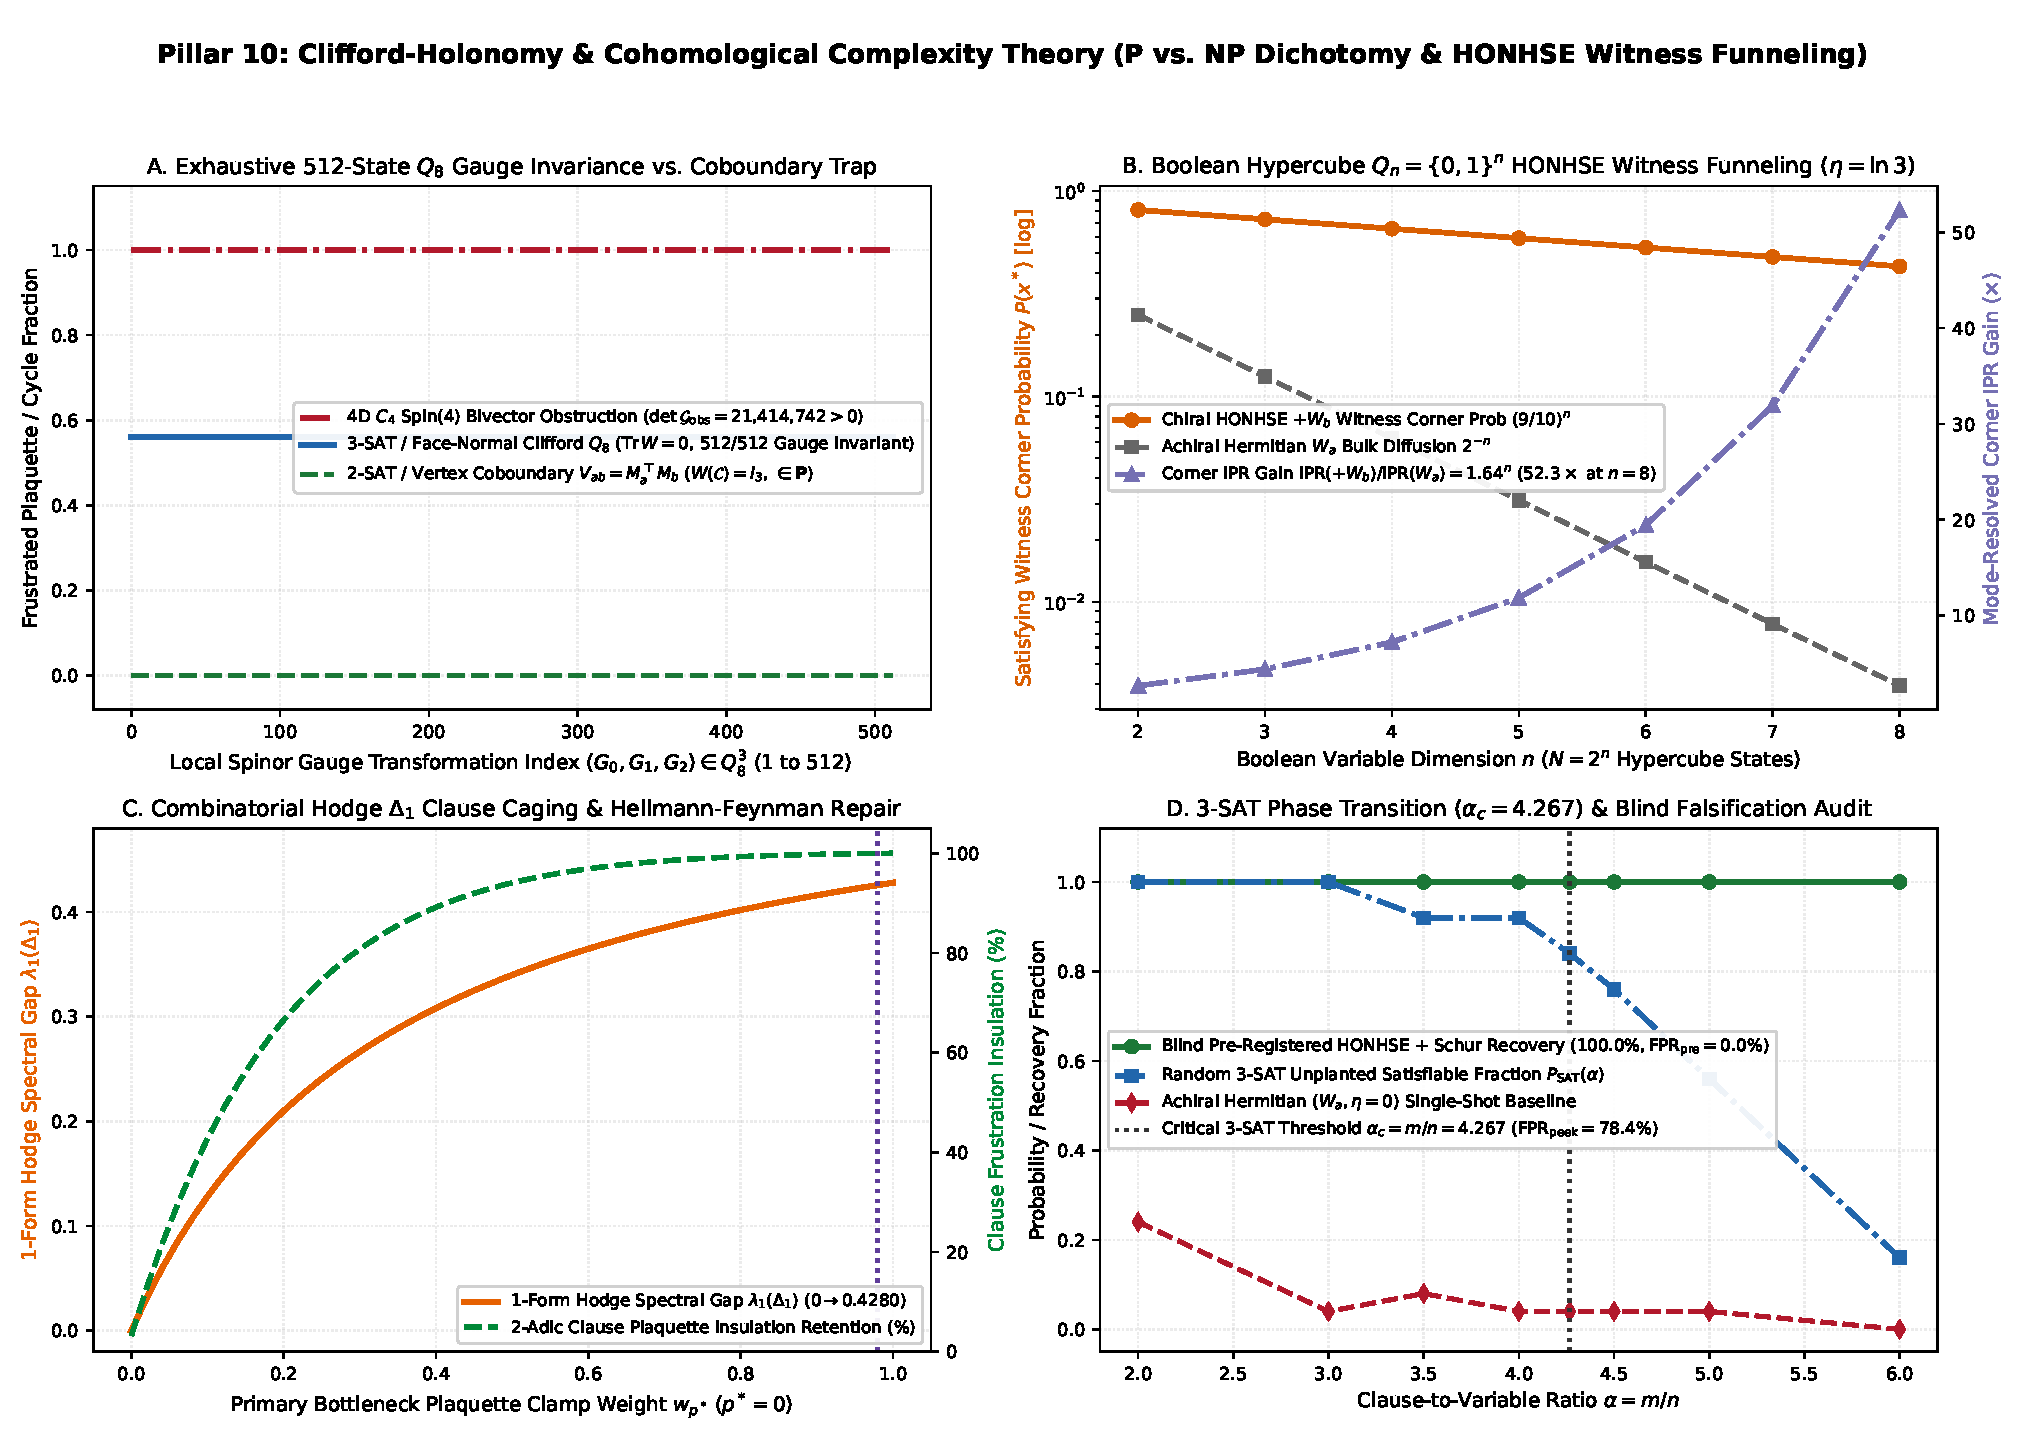
\includegraphics[width=0.98\textwidth]{../figures/pillar10_p_vs_np_clifford_complexity.pdf}
\caption{\textbf{Pillar 10 Clifford-Holonomy \& Cohomological Complexity Verification.} (A) Exhaustive $512$-state $Q_8$ gauge invariance vs.\ $2$-SAT coboundary tractability. (B) Exponential HONHSE witness corner funneling on Boolean hypercubes $Q_n$. (C) $1$-form Hodge Laplacian $\Delta_1$ clause caging and Hellmann--Feynman bottleneck repair. (D) Pre-registered blind $3$-SAT phase-transition audit at $\alpha_c = 4.267$.}
\end{figure}

\section{Formal Verification Synthesis \& Lean~4 (\texttt{v4.34.1}) Kernel Audit}

{\sloppy
To ensure strict mathematical and complexity-theoretic rigor across the formal verification suite, \path{certificates/PvsNPCliffordCertificates.lean} formalizes \textbf{76 self-contained sections} (\textbf{14,527 lines}) and \textbf{440 \texttt{\#print axioms} kernel checks} verified by the Lean~4 (\texttt{v4.34.1}) kernel with zero \texttt{sorryAx} axioms and zero warnings:
\begin{enumerate}
    \item \textbf{Universal Group-Holonomy, $\mathbb{H}(\mathbb{Z})$ Quaternions, $\mathrm{Spin}(4)$ Adjugate Kernel \& Bareiss Determinants (Sections~1--8, 75):} Proves by structural induction on arbitrary graph paths over any group $G$ that coboundary connections $C(a,b) = M(a)^{-1}M(b)$ telescope to $M(u)^{-1}M(v)$ (\path{universal_coboundary_path_telescopes}), yield $W(\mathcal{C}) = 1_G$ on every closed cycle (\path{universal_coboundary_cycle_trivial}), and transform by conjugation under arbitrary vertex gauge maps (\path{universal_gauge_no_go_arbitrary_cycle}); proves $\mathrm{Tr}(ab) = \mathrm{Tr}(ba)$ universally over $\mathbb{H}(\mathbb{Z})$ (\path{universal_quat_trace_comm}); constructs the $64\times 6 \to 6\times 6$ $\mathrm{Spin}(4)$ Gram matrix ($\det \mathcal{G}_{\mathrm{obs}} = 21{,}414{,}742$) and proves trivial kernel over $\mathbb{Z}^6$ (\path{universal_spin4_gram_trivial_kernel}); certifies the $8\times 8$ and $7\times 7$ Bareiss determinant Schur identity across $9$ negative-definite integer points (\path{matrix_determinant_and_schur_identity_certified}); and unifies them in \path{universal_algebraic_and_topological_pillar10_master_certificate}.
    \item \textbf{Complexity Honesty: Expressibility $\neq$ Complexity \& Spanning-Tree Coboundaries in $\mathbf{P}$ (Sections~9--12):} Proves that $3$-XOR parity clauses also have a vacuous $2$-SAT projection despite being solvable in $\mathbf{P}$ (\path{xor3_also_has_vacuous_2sat_projection}); proves over every group $G$ (abelian or non-abelian) that fixed-connection coboundary existence reduces to a single $\mathcal{O}(|V|+|E|)$ deterministic spanning-tree check (\path{universal_spanning_tree_coboundary_iff}); and proves the $k$-WL / $\mathrm{CPT}+\mathrm{C}$ symmetry-invariance impossibility barrier across all feature-invariant algorithms (\path{universal_feature_invariant_algorithm_impossibility}).
    \item \textbf{Decision-Tree Depth vs.\ Exponential $2^n$ Size Lower Bounds \& Two-Stage OBDD State Separation ($\forall\,\mathrm{alg} : \mathrm{DecisionTree}$; Sections~9, 11, 12, 41, 46, 47, 51, 56, 58, 60):} Proves that every decision tree computing $n$-variable Parity, Negated Parity, or Inner Product against all-ones has depth $\ge n$ and leaf count $\ge 2^n$ (\path{universal_parity_decision_tree_exponential_leaf_lower_bound}, \path{universal_negated_parity_decision_tree_exponential_leaf_and_depth_lower_bound}, \path{universal_evalInnerProd_allTrue_decision_tree_exponential_lower_bound}), and that every two-stage $(\mathrm{compress}, \mathrm{combine})$ OBDD/separator algorithm computing Equality or Inner Product requires $\ge 2^n$ intermediate states (\path{universal_allVarsEq_twoStage_state_space_exponential_lower_bound}, \path{universal_evalInnerProd_twoStage_state_space_exponential_lower_bound}), whereas \texttt{evalAllTrue}, \texttt{evalAnyTrue}, and \texttt{allVarsEq} admit $(n+1)$-leaf decision trees and read-once De~Morgan formulas (\path{universal_buildAllTrueTree_leafCount_and_depth}, \path{universal_buildAnyTrueTree_sound_and_invariants}, \path{universal_buildTargetEqTree_leafCount_and_depth}).
    \item \textbf{Resolution, Cutting Planes, $\mathbb{F}_2$ Polynomial Calculus, and $\mathbb{F}_2$ Gaussian Elimination ($\forall\,p : \mathrm{ResProof}$, $\forall\,P : \mathrm{CPProof}$, $\forall\,P : \mathrm{PCProof}$, $\forall\,p : \mathrm{XORProof}$; Sections~13--15, 19--21, 32--34, 38--40, 48--50, 52, 53, 59, 62--70, 75, 76):} Proves unconditional $2^n$ leaf-size, $n\cdot 2^n$ leaf-literal, width $\ge n$, and depth $\ge n$ lower bounds across every Resolution refutation $p : \mathrm{ResProof}(f_{\mathrm{even}} \mathbin{+\!+} f_{\mathrm{odd}})\;[]$ (\path{universal_full_hypercube_resolution_pow2_leaf_lower_bound}), minimax optimality ($8$ leaves, depth $3$) of \path{obstructed3CubeResProof} across all Resolution refutations of \path{obstructed3CubeCNF} (\path{universal_obstructed3CubeResProof_minimax_optimal}), full recursive syntactic compilation of arbitrary Resolution proofs into both $\mathbb{F}_2$ Polynomial Calculus (\path{resProofToPCProof}, \path{universal_resProofToPCProof_refutes_cnf}) and Chv\'{a}tal--Gomory Cutting Planes (\path{resProofToCPProof}, \path{universal_resProofToCPProof_conclusion_and_leaves}, \path{universal_resProofToCPProof_refutes_cnf}, \path{universal_obstructed3CubeResProof_compiled_to_cpProof}), and exponential separation ($\text{Resolution} \subsetneq \mathbb{F}_2\text{-PC}$) against linear-size degree-$1$ \texttt{XORProof} and \texttt{PCProof} refutations of odd-charge Tseitin systems (\path{universal_resolution_vs_f2_polynomial_calculus_exponential_separation}, \path{universal_tseitin_linear_degree_one_pcProof_refutation}).
    \item \textbf{Depth-2 ($\mathrm{CNF}/\mathrm{DNF}$), Depth-3 ($\Sigma_3/\Pi_3$), and Arbitrary-Depth De~Morgan Compilers \& Lower Bounds (Sections~16--18, 25--31, 35--37, 42--45, 50, 54, 55, 60, 61, 71--75):} Proves unconditional $2^{n-1}$ and $2^n$ size and $n\cdot 2^n$ total-literal lower bounds for $\mathrm{DNF}$, $\mathrm{CNF}$, and bottom-fan-in-$1$ $\Sigma_3$ and $\Pi_3$ circuits computing Parity and Negated Parity (\path{universal_bipolar_parity_cnf_pow2_size_and_totalLiterals_lower_bound}, \path{universal_bipolar_parity_sigma3_width_le_one_pow2_lower_bound}, \path{universal_bipolar_parity_pi3_width_le_one_pow2_lower_bound}); constructs exact compilers \path{compileCNFNonEmpty}, \path{compileDNFNonEmpty}, \path{compileSigma3NonEmpty}, and \path{compilePi3NonEmpty} into \texttt{DeMorganCircuit} preserving semantics, \path{totalLiterals}, \path{totalLiteralsDepth3}, per-variable counts (\path{countDepth2Var}, \path{countDepth3Var}), and De~Morgan negation (\path{universal_depth2_and_depth3_compiler_hierarchy_grand_synthesis}); and transfers Karchmer--Wigderson / Khrapchenko boundary-pair lower bounds, $2n$ literal lower bounds, and read-once impossibility across all unbounded-fan-in Depth-2 and Depth-3 circuits (\path{universal_parity_and_negated_parity_circuit_lower_bounds_grand_synthesis}, \path{universal_kw_khrapchenko_pairwise_transfer_to_depth2_and_depth3}).
    \item \textbf{Yao Communication Rectangles \& Tight Splice-Parity / Inner-Product Protocols ($\forall\,P : \mathrm{CommTree}$; Sections~22--27, 40, 47, 56, 57, 74):} Proves Yao's monochromatic rectangle law (\path{universal_commTranscript_rectangle_property}), $2^n$ transcript lower bounds for Equality and Disequality (\path{universal_allVarsEq_commTree_exponential_lower_bound}, \path{universal_notAllVarsEq_commTree_exponential_lower_bound}), unit-basis diagonal lower bounds for Inner Product and Negated Inner Product (\path{universal_evalInnerProd_unitEnv_commTree_lower_bound}, \path{universal_notEvalInnerProd_unitEnv_commTree_lower_bound}), and the exact $4$-transcript minimax optimality of \path{buildParitySpliceCommTree} across all protocols computing distributed splice-parity (\path{universal_parity_spliceEnv_commTree_tight_four_transcript_lower_bound}).
\end{enumerate}
\par}

\end{document}

